\begin{figure}[h]
  \centering
    \begin{subfigure}[b]{0.49\textwidth}
      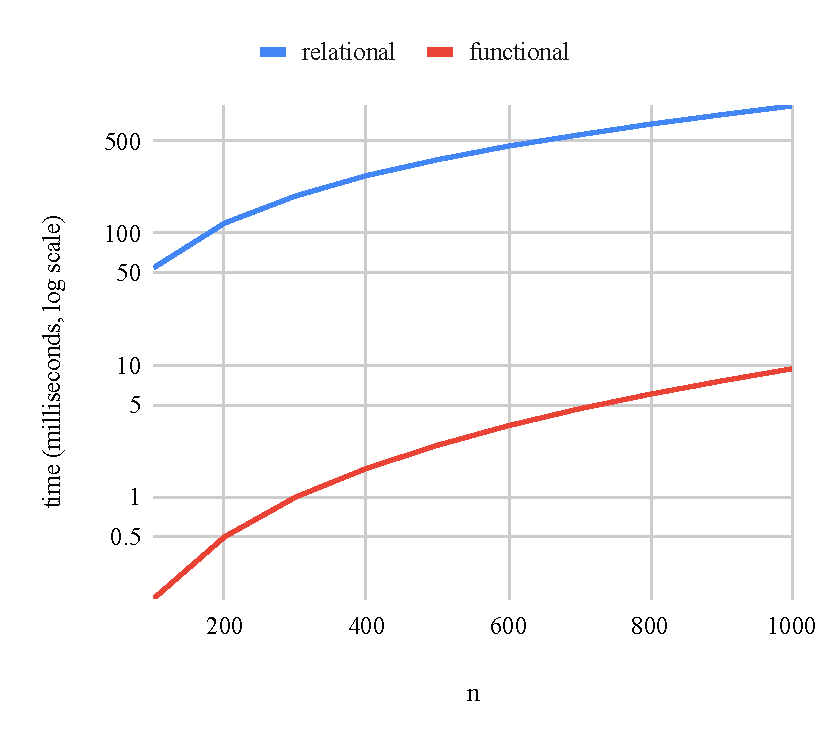
\includegraphics[width=\textwidth]{fig/muloIIO.pdf}
    \caption{Multiplication: \lstinline{mulo n 10 q}}
    \label{fig:mulo_IIO}
  \end{subfigure}
\hfill
    \begin{subfigure}[b]{0.49\textwidth}
      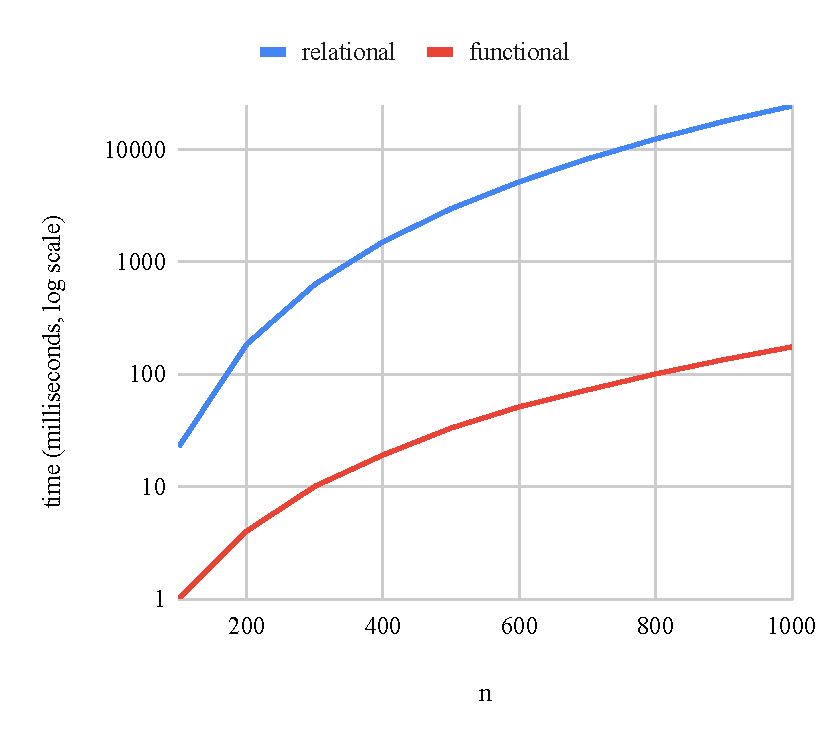
\includegraphics[width=1\textwidth]{fig/muloIOI.pdf}
    \caption{Division: \lstinline{mulo (n/10) q n}}
    \label{fig:mulo_IOI}
  \end{subfigure}

\hfill

    \begin{subfigure}[b]{0.49\textwidth}
      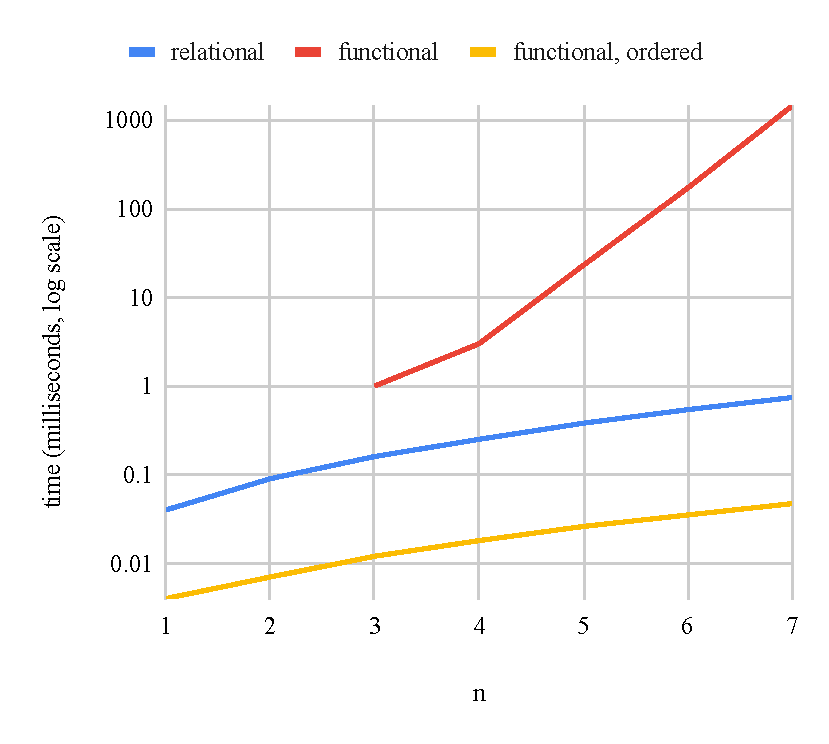
\includegraphics[width=\textwidth]{fig/muloIOO.pdf}
    \caption{Generation: \lstinline{take n (mulo 10 q r)}}
    \label{fig:mulo_IOO}
  \end{subfigure}
\hfill
  \begin{subfigure}[b]{0.45\textwidth}
    \begin{subfigure}[b]{\textwidth}
    \begin{lstlisting}[frame=tb]
let rec mul$^o$ x$^{g \rightarrow g}$ y$^{f \rightarrow g}$ z$^{f \rightarrow g}$ =
  (x$^{g \rightarrow g}$ ===    O /\ z$^{f \rightarrow g}$ ===    O) \/
  (x$^{g \rightarrow g}$ ===    S x$_1^{f \rightarrow g}$ /\
   add$^o$ y$^{f \rightarrow g}$ z$_1^{f \rightarrow g}$ z$^{f \rightarrow g}$ /\
   mul$^o$ x$_1^{g \rightarrow g}$ y$^{g \rightarrow g}$ z$_1^{g \rightarrow g}$
   )
    \end{lstlisting}
    \caption{Inefficient mode}
    \label{fig:mult_modded_bad}
  \end{subfigure}
  \hfill

    \begin{subfigure}[b]{\textwidth}
    \begin{lstlisting}[frame=tb]
let rec mul$^o$ x$^{g \rightarrow g}$ y$^{f \rightarrow g}$ z$^{f \rightarrow g}$ =
  (x$^{g \rightarrow g}$ ===    O /\ z$^{f \rightarrow g}$ ===    O) \/
  (x$^{g \rightarrow g}$ ===    S x$_1^{f \rightarrow g}$) /\
   mul$^o$ x$_1^{g \rightarrow g}$ y$^{f \rightarrow g}$ z$_1^{f \rightarrow g}$ /\
   add$^o$ y$^{g \rightarrow g}$ z$_1^{g \rightarrow g}$ z$^{f \rightarrow g}$
    \end{lstlisting}
    \caption{Efficient mode}
    \label{fig:mult_modded_good}
  \end{subfigure}
  \end{subfigure}

  \caption{Execution times of the multiplication relation}
  \label{fig:mulo_time}
\end{figure}
